\section{1174057 Alit Fajar Kurniawan}
\subsection{Teori}
\begin{enumerate}
\item Jelaskan kenapa file suara harus di lakukan MFCC
\par  MFCC ( Mel Frequency Cepstral Coefficients ) merupakan koefisien yang merepresentasikan audio. Ekstraksi ciri dalam proses ini ditandai dengan pengubahan data suara menjadi data citra berupa spektrum gelombang. Diharuskan melakukan MFCC kepada objek suara agar suara dapat diubah ke dalam bentuk data matrix dimana telah dilakukan ekstraksi oleh MFCC kemudian direalisasikan sebagai data matrix. Suara tersebut menjadi vektor yang nantinya akan diolah jadi outputan.

\begin{figure}[H]
\centering
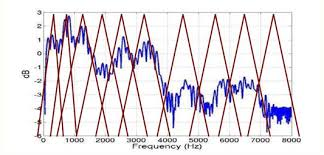
\includegraphics[scale=0.5]{figures/1174057/chapter6/1.jpg}
\caption{Ilustrasi MFCC}
\label{Ilustrasi MFCC}
\end{figure}

\par Penjelasan dari gambar diatas, digambarkan sebuah bingkai dari klip suara bernyanyi untuk pengujian yang sama. Dengan menggunakan jendela Hamming, harmonik dalam respons frekuensi jauh lebih tajam.Untuk bingkai input terdiri dari 3 periode fundamental yang identik, maka respons frekuensi magnitudo akan dimasukkan 2 nol antara setiap dua titik tetangga dari respons frekuensi dari periode fundamental tunggal. Dengan kata lain, harmonik dari respons frekuensi umumnya disebabkan oleh periode fundamental berulang dalam bingkai.

\item Jelaskan konsep dasar neural network
\par Neural Network merupakan kategori ilmu Soft Computing. Neural Network mengambil kemampuan dari otak manusia yang mampu memberikan stimulasi, melakukan proses, dan memberikan output. Output atau hasil didapatkan dari variasi stimulasi dan proses yang terjadi pada otak manusia. Kemampuan manusia dalam memproses informasi adalah hasil kompleksitas proses di dalam otak manusia. Misalnya, yang terjadi pada anak-anak, mereka mampu belajar untuk melakukan pengenalan meskipun mereka tidak mengetahui algoritma apa yang digunakan. 
\begin{figure}[H]
\centering
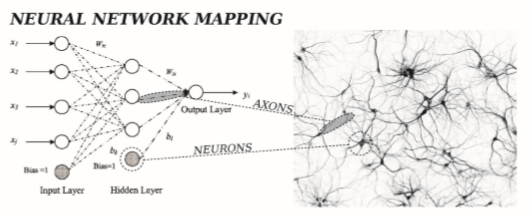
\includegraphics[scale=0.5]{figures/1174057/chapter6/2.PNG}
\caption{Konsep Dasar Neural Network}
\label{Konsep Dasar Neural Network}
\end{figure}

\item Jelaskan konsep pembobotan dalam neural network

\par Sebuah Neural Network dikonfigurasi untuk aplikasi tertentu, seperti pengenalan pola atau klasifikasi data. Terjadi penglibatan dalam penyesuaian koneksi sinaptik yang ada antara neuron ketika melakukan penyempurnaan dengan proses pembelajaran. Penyesuaian nilai bobot yang ada pada tiap konektivitas baik dari input, neuron maupun output disinkronkan dengan penyesuaian koneksi sinaptik antar neuron itu sendiri. 
\begin{figure}[H]
\centering
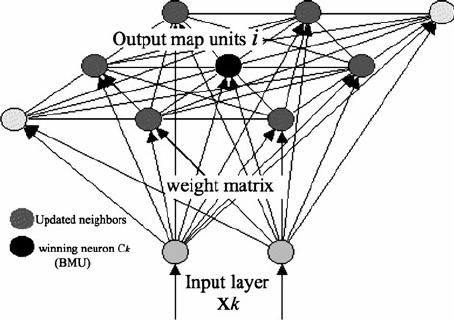
\includegraphics[scale=0.4]{figures/1174057/chapter6/3.png}
\caption{Pembobotan Neural Network}
\label{Pembobotan Neural Network}
\end{figure}		

\item Jelaskan konsep fungsi aktifasi dalam neural network
\par Fungsi aktivasi pada neural network berfungsi layaknya sinapsis pada neuron manusia. Dimana pada neural network, fungsi aktivasi sebagai penentu aktivasi dari sebuah nilai input-an yang sebelumnya telah dihitung pada hidden layer. 
\begin{figure}[H]
\centering
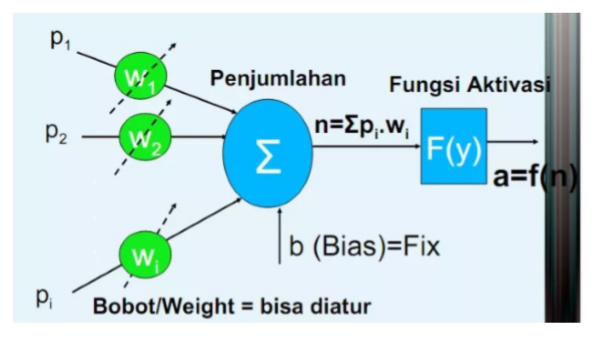
\includegraphics[scale=0.4]{figures/1174057/chapter6/4.PNG}
\caption{fungsi aktifasi dalam neural network}
\label{fungsi aktifasi dalam neural network}
\end{figure}	

\item Jelaskan cara membaca hasil plot dari MFCC
\par Pada sebuah grafik hasil plot dari MFCC gambar \ref{Ilustrasi MFC}, terdapat 2 sumbu yaitu x dan y. Sumbu Y merupakan waktu atau durasi dari sebuah suara/musik/lagu, sedangkan sumbu X merupakan frekuensi dari suara yang dihasilkan, dan hasilnya merupakan desibel/power. Desibel yang dihasilkan memiliki range warna yang berbeda-beda. Range warna dari desibel adalah mulai dari biru tua hingga coklat tua. Range warna biru merupakan suara yang tidak dapat didengar manusia dan coklat merupakan suara yang dapat dapat didengar manusia.
\begin{figure}[H]
\centering
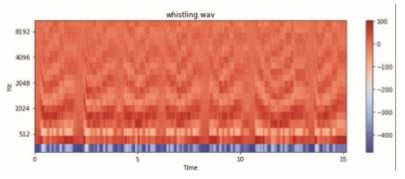
\includegraphics[scale=0.4]{figures/1174057/chapter6/5.PNG}
\caption{Membaca hasil plot}
\label{Membaca hasil plot}
\end{figure}

\item Jelaskan apa itu one-hot encoding
\par Proses di mana variabel kategorikal dikonversi menjadi bentuk yang dapat disediakan untuk algoritma ML untuk melakukan pekerjaan yang lebih baik dalam prediksi.
\begin{figure}[H]
\centering
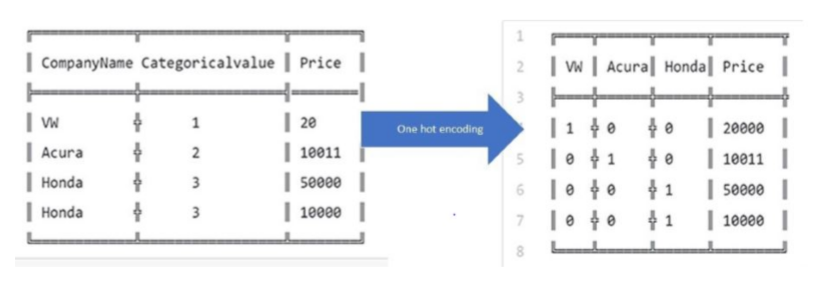
\includegraphics[scale=0.3]{figures/1174057/chapter6/6_1.PNG}
\caption{One-Hot Encoding }
\label{One-Hot Encoding }
\end{figure}

\par Nilai kategoris mewakili nilai numerik dari entri dalam dataset. Dicontohkan apabila ada perusahaan lain dalam dataset, Ketika jumlah entri unik meningkat, nilai kategoris juga meningkat secara proporsional. Tabel sebelumnya hanyalah representasi. Pada kenyataannya, nilai-nilai kategorikal mulai dari 0 sampai dengan kategori N-1. Inimerupakan bentuk organisasi yang didefinisikan dengan VW¿ Acura¿ Honda berdasarkan pada nilai-nilai kategorikal. Rata-rata VW dan Honda adalah Acura, dengan menggunakan satu one-hot encoding untuk melakukan ”binarisasi” kategori dan memasukkannya sebagai fitur untuk melatih model sehingga memberikan hasil yang sesuai.

\item Jelaskan apa fungsi dari np.unique dan to categorical dalam kode program
\par np.unique berfungsi Untuk mengekstaksi elemen-elemen unik (tertentu) dalam array.
\begin{figure}[H]
\centering
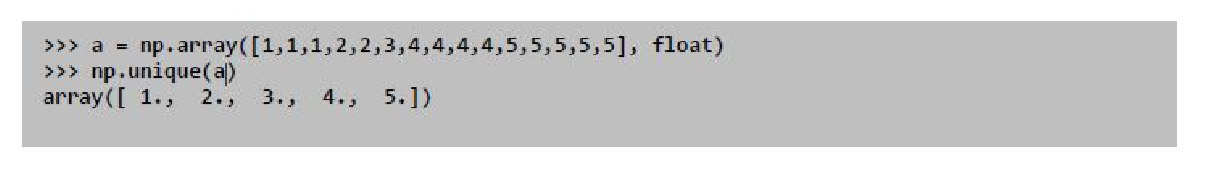
\includegraphics[scale=0.4]{figures/1174057/chapter6/7_1.PNG}
\caption{np.unique}
\label{np.unique}
\end{figure}

\par To categorical Berfungsi untuk mengubah vektor kelas yang berupa integer ( number ) menjadi matriks kelas biner.
\begin{figure}[H]
\centering
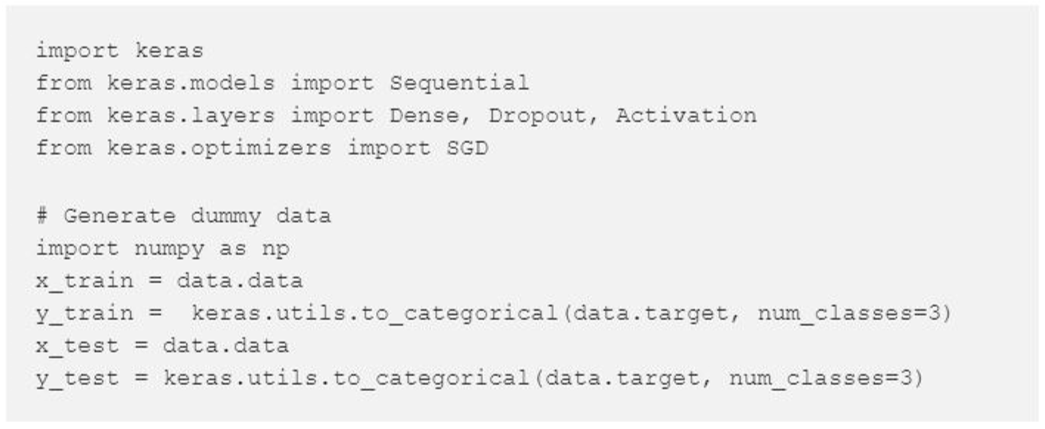
\includegraphics[scale=0.4]{figures/1174057/chapter6/7_2.PNG}
\caption{To categorical}
\label{To categorical}
\end{figure}

\item Jelaskan apa fungsi dari Sequential dalam kode program
\par Sebuah jenis model yang digunakan dalam perhitungan ataupun code program yang direalisasikan. Neural Networks Sequential membangun fitur tingkat tinggi melalui lapisannya yang berurutan. Sequential juga suatu proses dimana membandingkan setiap per elemen larik satu per satu secara berurutan, mulai dari elemen pertama, sampai dengan elemen terakhir atau elemen yang dicari sudah ditemukan. 
\begin{figure}[H]
\centering
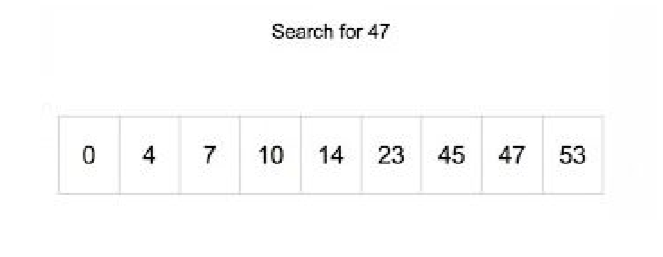
\includegraphics[scale=0.4]{figures/1174057/chapter6/8.PNG}
\caption{fungsi dari Sequential}
\label{fungsi dari Sequential}
\end{figure}
\par Pada gambar diatas mendefinisikan pencarian terhadap angka 47 dimana hasilnya tetap diurutkan sesuai dengan elemennya.
\end{enumerate}

\subsection{Praktek}
\begin{enumerate}

\item Jelaskan isi dari data GTZAN Genre Collection dan data dari freesound

\par Sebelumnya teman-teman bisa mendownload terlebih dahulu data nya pada google untuk melakukan pengujian agar dapat berjalan. Pada GTZAN Genre Collection merupakan berupa data musik yang sudah di folderkan berdasarkan genre lagunya. Datasets lagu atau suara yang terisi dari 10 gendre musik yang tersimpan dalam 10 folder yaitu folder yaitu classical, disco, pop, country, hiphop, blues, jazz, rock, metal, dan reggea. untuk menguji hasil pengolahan data tersebut dengan menggunakan metode mfcc.
\begin{verbatim}
import librosa #import librosa tang digunakan untuk fungsi mfcc
import librosa.feature #import librosa featuse dan pada baris
import librosa.display #import librosa display
import glob #import glob 
import numpy as np #insert numpy untuk pengolahan data menjadi vektor
import matplotlib.pyplot as plt #import matplotlib untuk melakukan ploting
from keras.models import Sequential 
from keras.layers import Dense, Activation
from keras.utils.np_utils import to_categorical

# In[1]: membuat fungsi mfcc untuk melakukan pengujian
def display_mfcc(song): #membuat fungsi mfcc (display_mfcc) dan terdapat variabel Y
    y, _ = librosa.load(song) #method librosa load 
    mfcc = librosa.feature.mfcc(y) # method librosa featurea mfcc

    plt.figure(figsize=(10, 4)) #membuat flot figure dengan ukuran 10 banding 4
    librosa.display.specshow(mfcc, x_axis='time', y_axis='mel') #data librosa display dengan variabel x nya yaitu waktu dan y yaitu mel atau Hz
    plt.colorbar() #plot warna 
    plt.title(song) #plot judul 
    plt.tight_layout()
    plt.show() #plot di tampilkan
\end{verbatim}
\begin{figure}[H]
\centering
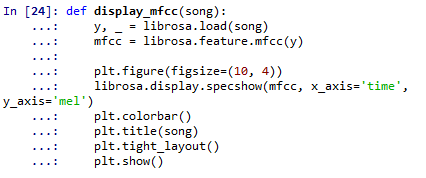
\includegraphics[scale=0.5]{figures/1174057/chapter6/p1.PNG}
\caption{Praktek 1}
\label{Praktek 1}
\end{figure}

\item Jelaskan perbaris kode program dengan kata kata dan dilengkapi ilustrasi gambar fungsi dari display mfcc
\begin{verbatim}
# In[2]: cek fungsi
display_mfcc('C:/Users/Alit/Desktop/KB3B/genres/hiphop/hiphop.00050.au') 
#untuk mendisplay tampilan glombang suara dari file 266093 stereo-surgeon kick-loop-5.wav menggunakan metode mfcc
# In[2]: cek fungsi
display_mfcc('C:/Users/Alit/Desktop/KB3B/genres/jazz/jazz.00050.au')
# In[2]: cek fungsi
display_mfcc('C:/Users/Alit/Desktop/KB3B/genres/pop/pop.00050.au')
# In[2]: cek fungsi
display_mfcc('C:/Users/Alit/Desktop/KB3B/genres/reggae/reggae.00050.au')
# In[2]: cek fungsi
display_mfcc('C:/Users/Alit/Desktop/KB3B/genres/rock/rock.00050.au')
\end{verbatim}

    	   	\begin{figure}[H]
				\centering
				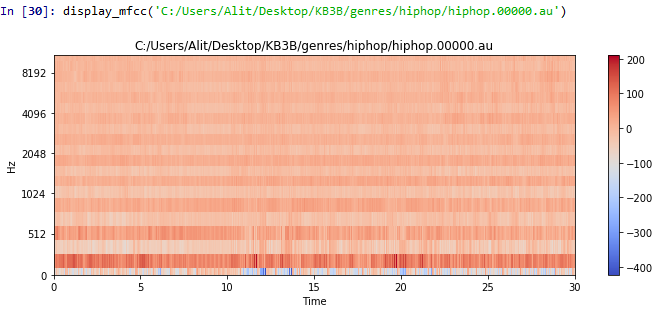
\includegraphics[scale=0.5]{figures/1174057/chapter6/p2.PNG}
				\caption{Praktek}
				\label{Praktek}
			\end{figure}
	
    	   	\begin{figure}[H]
				\centering
				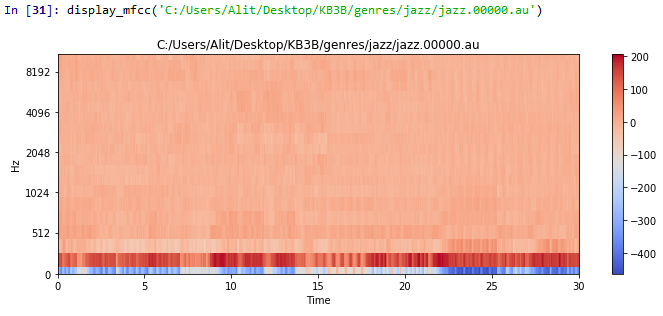
\includegraphics[scale=0.5]{figures/1174057/chapter6/p2_1.PNG}
				\caption{Praktek}
				\label{Praktek}
			\end{figure}

		\subitem Untuk hasil contoh selanjutnya bisa melakukan pengujian sendiri

		\item Jelaskan perbaris kode program dengan kata-kata dan dilengkapi ilustrasi gambar fungsi dari extract features song(). Jelaskan juga mengapa yang diambil 25.000 baris pertama?

\begin{verbatim}
# In[3]:
def extract_features_song(f): #nama extract features song yang nantinya akan di gunakan pada fungsi yang lainya
    y, _ = librosa.load(f) #membuat variabel y dengan method librosa load

    mfcc = librosa.feature.mfcc(y) #membuat variabel baru mfcc dengan isi librosa features mfcc dengan isi variabel y

    mfcc /= np.amax(np.absolute(mfcc)) #variabel mfcc dengan isian np.max

    return np.ndarray.flatten(mfcc)[:25000] #membuat array dari data tersebut merupakan data 25000 data pertama
\end{verbatim}

		\par kenapa data 25000 pertama yang digunakan karena data tersebut digunakan sebagai data testing semakin besar data testing yang di gunakan maka semakin akurat hasil kecerdasan buatan yang dihasilkan. tapi sebenarnya data tersebut relatif bisa lebih besar atau lebih kecil tergantung pada komputer masing masing.

		\item Jelaskan perbaris kode program dengan kata-kata dan dilengkapi ilustrasi gambar fungsi dari generate features and labels().
		\par Lihatlah pada praktek kode program berikut, dan sudah ada penjelasan pada kode program 
		\begin{verbatim}
		# In[4]:
		def generate_features_and_labels(): #pendefinisian nama fungsi yaitu generate features and labels
		    all_features = [] #variabel baru dengan array all features
		    all_labels = [] #variabel baru dengan array all labels

		    genres = ['blues', 'classical', 'country', 'disco', 'hiphop', 'jazz', 'metal', 'pop', 'reggae', 'rock'] #kemudian mendefinisikan isian label untuk gendre
		    for genre in genres:
		        sound_files = glob.glob('genres/'+genre+'/*.au')
		        print('Processing %d songs in %s genre...' % (len(sound_files), genre))
		        for f in sound_files:
		            features = extract_features_song(f)
		            all_features.append(features)
		            all_labels.append(genre)

		    # convert labels to one-hot encoding cth blues : 1000000000 classic 0100000000
		    label_uniq_ids, label_row_ids = np.unique(all_labels, return_inverse=True)#ke integer
		    label_row_ids = label_row_ids.astype(np.int32, copy=False)
		    onehot_labels = to_categorical(label_row_ids, len(label_uniq_ids))#ke one hot
		    return np.stack(all_features), onehot_labels
		\end{verbatim}

		\item Jelaskan dengan kata dan praktek kenapa penggunaan fungsi generate features and labels() sangat lama ketika meload dataset genre. Tunjukkan keluarannya dari komputer sendiri dan artikan maksud setiap luaran yang didapatkan.
		\par dalam melakukan penggunaan fungsi generate features and labels() membutuhkan waktu yang lama dikarenakan mesin membaca file secara satu persatu dari total jumlah 100 file yang dibaca ditambah lagi dengan proses perubahan data yang dilakukan oleh mesin dari bentuk suara menjadi bentuk vektor.
		\begin{verbatim}
		# In[5]: passing parameter dari fitur ekstraksi menggunakan mfcc
		features, labels = generate_features_and_labels()
		\end{verbatim}
    	   	\begin{figure}[H]
				\centering
				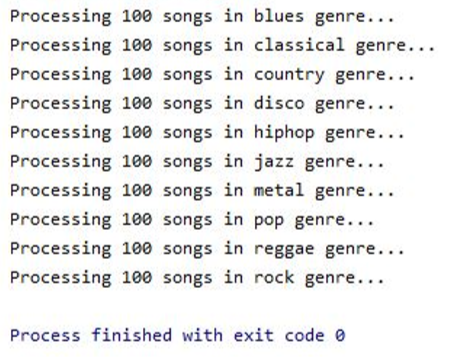
\includegraphics[scale=0.4]{figures/1174057/chapter6/p5.PNG}
				\caption{Praktek 2 Contoh 5}
				\label{Praktek 2 Contoh 5}
			\end{figure}

		\item Jelaskan kenapa harus dilakukan pemisahan data training dan data set sebesar 80 persen? Praktekkan dengan kode dan Tunjukkan keluarannya dari komputer sendiri dan artikan maksud setiap luaran yang didapatkan.
		\par berikut kode program yang merupakan kode untuk membagi data sebanyak 80 persen untuk data training maka data musik tadi yang total jumlahnya 1000 akan di bagi dua untuk data training sebanyak 800 dan 200 untuk data testing.
		\begin{verbatim} 
		# In[6] fitur ekstraksi
		training_split = 0.8
		\end{verbatim}
		\item Praktekkan dan jelaskan masing-masing parameter dari fungsi Sequential().Tunjukkan keluarannya dari komputer sendiri dan artikan maksud setiap luaran yang didapatkan.
		\par Fungsi sequential itu sendiri digunakan untuk melakukan pengolahan data inputan sesuai dengan fungsi yang ada pada fungsi sequential pada fungsi sequential kali ini menggunakan dua fungsi se\par quential meng-compile data dari 100 neuron atau dari 1 folder file dengan menggunakan fungsi relu dan softmax untuk menghasilkan outputan yang sesuai dengan keriteria.

		\begin{verbatim}
		# In[7]: membuat seq NN, layer pertama dense dari 100 neurons
		model = Sequential([
		    Dense(100, input_dim=np.shape(train_input)[1]),
		    Activation('relu'),
		    Dense(10),
		    Activation('softmax'),
		    ])
		\end{verbatim}

		\item Praktekkan dan jelaskan masing-masing parameter dari fungsi compile().Tunjukkan keluarannya dengan fungsi summary dari komputer sendiri dan artikan maksud setiap luaran yang didapatkan.
		\par yaitu fungsi compile yang digunakan untuk mengetahui parameter yang digunakan dari data yang telah diolah untuk caranya dapat menggunakan codingan sebagai berikut, pada gambar tersebut memunculkan parameternya berapasaja dan total parameter yang digunakan.

		\begin{verbatim}
		# In[8]: 
		model.compile(optimizer='adam',
		              loss='categorical_crossentropy',
		              metrics=['accuracy'])
		print(model.summary())
		\end{verbatim}
    	   	\begin{figure}[H]
				\centering
				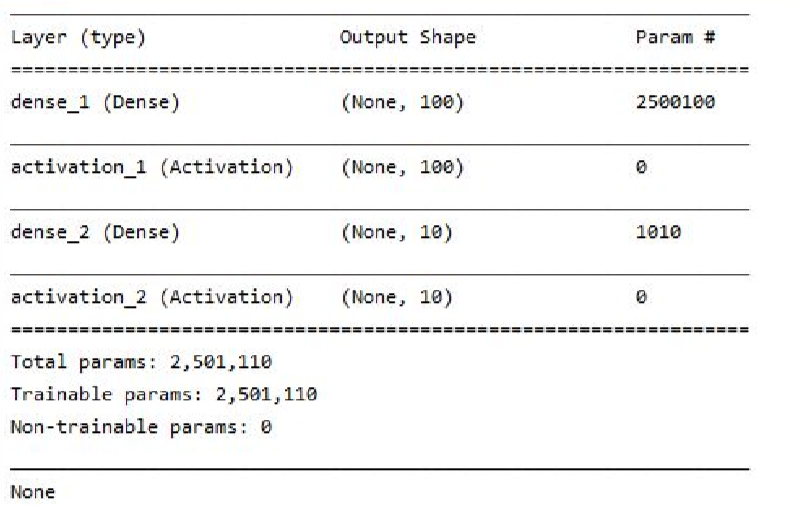
\includegraphics[scale=0.4]{figures/1174057/chapter6/p8.PNG}
				\caption{Praktek 2 Contoh 8}
				\label{Praktek 2 Contoh 8}
			\end{figure}

		\item Praktekkan dan jelaskan masing-masing parameter dari fungsi fit().Tunjukkan keluarannya dari komputer sendiri dan artikan maksud setiap luaran yang didapatkan.
		\par Pada fungsi ini dilakukan pengolahan data dari 10 label tadi atau 10 file dataset tadi kemudian dihitung tingkat akurasi masing masing dan tingkat kegagalan atau loss data darisetiap file tersebut caranya dengan melakukan codingan berikut. pada gambar tersebut menunjukan 10 pengolahan data untuk menentukan nilai akurasi dan loss dari data tersebut dan selanjutnya dilakukan fingsi evaluasi.

		\begin{verbatim}
		# In[9]:
		model.fit(train_input, train_labels, epochs=10, batch_size=32,
		          validation_split=0.2)
		\end{verbatim}
    	   	\begin{figure}[H]
				\centering
				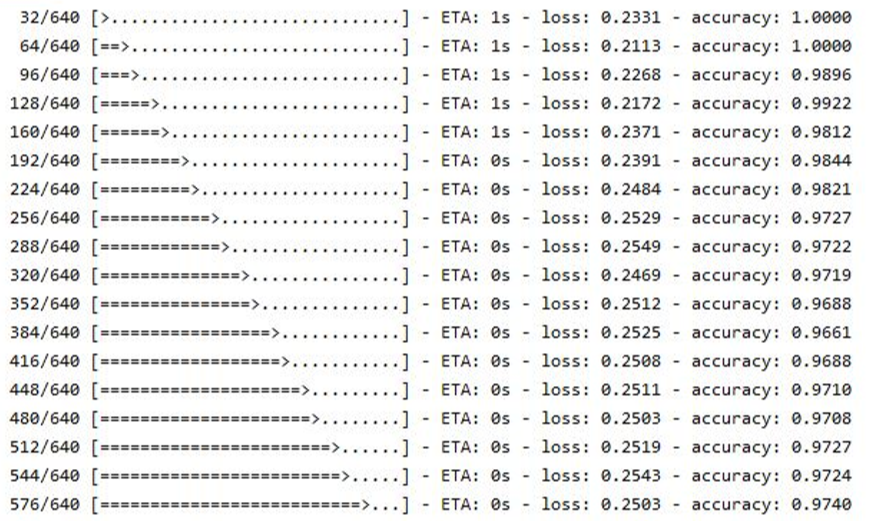
\includegraphics[scale=0.4]{figures/1174057/chapter6/p9.PNG}
				\caption{Praktek 2 Contoh 9}
				\label{Praktek 2 Contoh 9}
			\end{figure}

		\item Praktekkan dan jelaskan masing-masing parameter dari fungsi evaluate().Tunjukkan keluarannya dari komputer sendiri dan artikan maksud setiap luaran yang didapatkan.
		\par pada fungsi ini dilakukan evaluasi terhadap datayang telah di runing sebelummnya untuk lebih jelasnya dapat di lihat codingan tersebut pada codingan tersebut dilakukan evaluasi pada tingkat kegagalan dan akurasi kebenaran maka hasilnya munculkan hasil evaluasi dari 10 proses dari setiap gendre yaitu akurasi sebesar 51 persen dan loss data sebesar 1.4105 data.

		% \begin{verbatim}
		% 	# In[10]
		% 	loss, acc = model.evaluate(test_input, test_labels, batch_size=32)

		% 	# In[]: 
		% 	print("Done!")
		% 	print("Loss: %.4f, accuracy: %.4f" % (loss, acc))
		% \end{verbatim}
    	   	\begin{figure}[H]
				\centering
				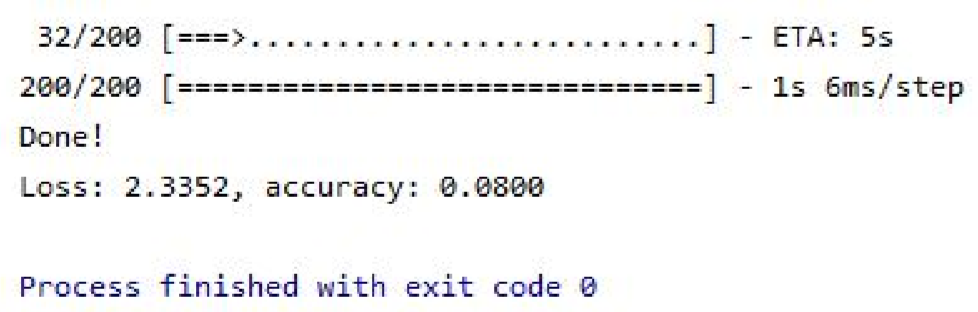
\includegraphics[scale=0.4]{figures/1174057/chapter6/p10.PNG}
				\caption{Praktek 2 Contoh 10}
				\label{Praktek 2 Contoh 10}
			\end{figure}

		\item Praktekkan dan jelaskan masing-masing parameter dari fungsi predict().Tunjukkan keluarannya dari komputer sendiri dan artikan maksud setiap luaran yang didapatkan.
		\par fungsi predic merupakan fungsi untuk membandingkan tingkat akurasi pada setiap label yang sepuluh tadi maka data akan di sandingkan ke masing masing tingkat akurasinya, yang akurasinya paling tinggi maka itulah jawaban untuk setiap inputan yang dilakukan.

		% \begin{verbatim}
		% 	# In[]: 
		% 	model.predict(test_input[:1])
		% \end{verbatim}
    	   	\begin{figure}[H]
				\centering
				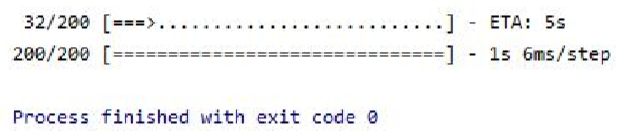
\includegraphics[scale=0.4]{figures/1174057/chapter6/p11.PNG}
				\caption{Praktek 2 Contoh 11}
				\label{Praktek 2 Contoh 11}
			\end{figure}
	\end{enumerate}

    \subsection{Plagiarisme}
    	   	\begin{figure}[H]
				\centering
				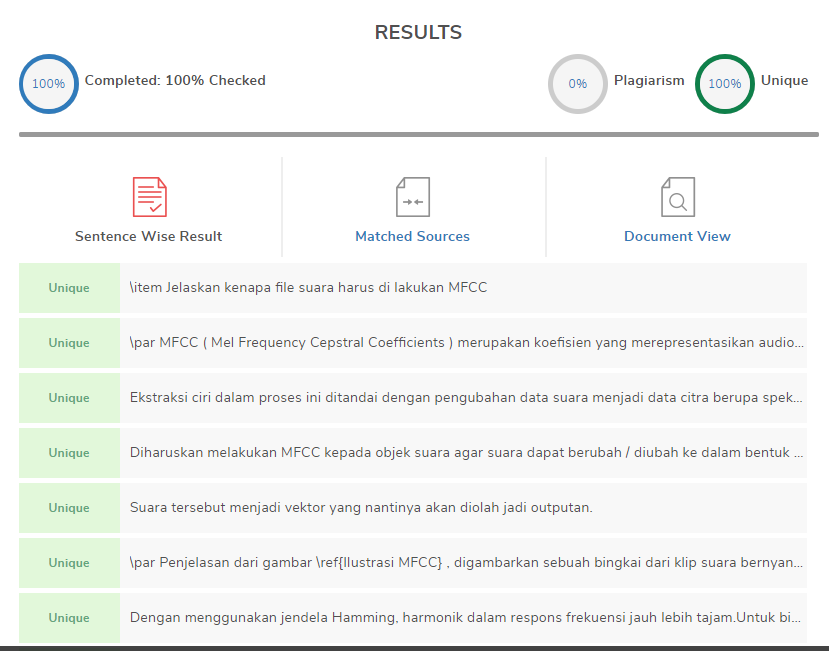
\includegraphics[scale=0.5]{figures/1174057/chapter6/plagiat.PNG}
				\caption{Plagiarisme}
				\label{Plagiarisme}
			\end{figure}